\documentclass[11pt]{article}
\usepackage[margin=1in]{geometry}
\usepackage[T1]{fontenc}
\usepackage{lmodern}
\usepackage{booktabs}
\usepackage{longtable}
\usepackage{float}
\usepackage{amsmath}
\usepackage{setspace}
\usepackage{tikz}
\usetikzlibrary{positioning,arrows.meta}
\input{glyphtounicode}
\pdfgentounicode=1
\hyphenpenalty=10000
\exhyphenpenalty=10000
\emergencystretch=3em
\setstretch{1.12}
\pagestyle{plain}

\begin{document}

\begin{center}
{\Large\bfseries Recognition Programs Improve Performance:\\ A Meta-Analysis of 61 Samples\par}
\vspace{0.8em}
{\bfseries SYNTHETIC TEST PAPER, NOT REAL RESEARCH\par}
\vspace{0.8em}
Avery Placeholder and Jordan Example\\
Department of Imaginary Management, Fictional State University\\
{\small (All authors, primary studies, firms, and data sets in this paper are fictional.)}
\end{center}

\begin{abstract}
\noindent Prior studies disagree about whether workplace recognition programs pay off, and the disagreement is sharpest in small firms. We meta-analyze 180 effect sizes from 61 samples (N = 45,960) and find that recognition programs improve unit and firm performance (corrected rho = .12). The effect is consistently positive across settings, which resolves the inconsistency in prior findings. Our second main finding is that the effect holds even in small firms. A meta-analytic structural equation model traces the effect through employee engagement, voluntary turnover, and customer satisfaction. Moderator analyses identify two boundary conditions that lie in program design: manager training and public delivery.

\medskip
\noindent\textit{Keywords:} employee recognition, firm performance, meta-analysis, MASEM
\end{abstract}

\section{Introduction}

Firms spend heavily on programs that recognize employees: awards, public thanks, service milestones, and small non-cash rewards. Whether these programs are associated with better unit and firm performance is still debated. Some studies of recognition and return on assets (ROA) report clear positive associations (see the Cordero and Hollis 1997 and Zeller and Kaur 2014 rows of Table 1), while others report associations near zero (the Pacheco 1994 and Valcourt 2009 rows). The disagreement is sharpest in small firms, where the few available studies point in different directions and where managers have the least slack to spend on programs that may not pay off.

This paper pools the evidence. We meta-analyze 180 effect sizes from 61 samples of units and firms, covering published and unpublished work from 1990 to 2024. The paper makes three contributions. First, and most important, it shows that the relationship between recognition and performance generalizes across settings, including small firms, where prior findings disagreed; this resolves the inconsistent findings of earlier work. Second, it uses meta-analytic structural equation modeling (MASEM) to trace the pathway that links recognition to ROA through employee engagement, voluntary turnover, and customer satisfaction. Third, it identifies boundary conditions of the relationship that lie in how programs are designed and delivered.

\section{Theory and Hypotheses}

Recognition signals to employees that their effort is seen and valued. Social exchange accounts hold that employees who feel valued reciprocate with engagement and discretionary effort, and that engaged employees are less likely to quit. Lower turnover preserves firm-specific knowledge and service relationships, which should show up in customer satisfaction and, in the end, in ROA. These arguments lead to three hypotheses.

\medskip
\noindent\textit{Hypothesis 1.} Recognition program intensity is positively related to unit and firm ROA.

\noindent\textit{Hypothesis 2.} Employee engagement, voluntary turnover, and customer satisfaction link recognition program intensity to ROA.

\noindent\textit{Hypothesis 3.} The relationship between recognition and ROA is stronger when managers are trained to give recognition and when recognition is delivered in public.

\section{Method}

\subsection{Literature search}

We searched ABI/INFORM Global, Business Source Complete, APA PsycInfo, the Web of Science Core Collection, ProQuest Dissertations and Theses Global, SSRN, and the Academy of Management Proceedings for work dated from January 1990 through December 2024. The last search ran on 20 December 2024. Appendix A gives the full search string used in each database. The dissertation database, SSRN, and the Academy of Management Proceedings were included to find unpublished work: dissertations, working papers, and conference papers. Records from all sources are counted together in Figure 1. Section 4.4 compares published and unpublished effect sizes.

\subsection{Inclusion rules and screening}

Before coding began, we wrote down the inclusion rules and the coding manual. A study was eligible if it (a) reported on a sample of employees, units, or firms, (b) measured the presence or intensity of a recognition program, (c) measured unit or firm ROA, and (d) reported a correlation between the two or a statistic that can be converted to one. Two authors screened every title and abstract independently and agreed on 94 percent of screening decisions; they resolved disagreements by discussion. Figure 1 shows the flow of records in the PRISMA 2020 format (Page et al. 2021).

\begin{figure}[H]
\centering
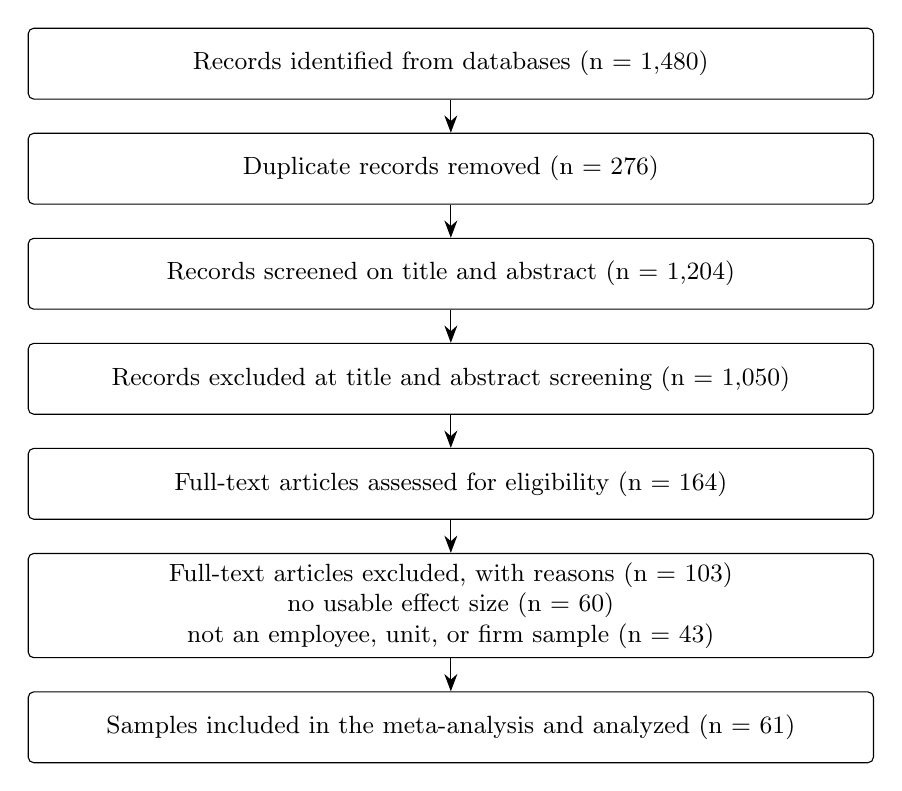
\begin{tikzpicture}[
  box/.style={draw, rounded corners=2pt, align=center, text width=10.5cm, minimum height=0.9cm, font=\small},
  arr/.style={-{Stealth[length=2.2mm]}},
  node distance=0.42cm]
\node[box] (id) {Records identified from databases (n = 1,480)};
\node[box, below=of id] (dup) {Duplicate records removed (n = 276)};
\node[box, below=of dup] (scr) {Records screened on title and abstract (n = 1,204)};
\node[box, below=of scr] (exs) {Records excluded at title and abstract screening (n = 1,050)};
\node[box, below=of exs] (ft) {Full-text articles assessed for eligibility (n = 164)};
\node[box, below=of ft] (exf) {Full-text articles excluded, with reasons (n = 103)\\ no usable effect size (n = 60)\\ not an employee, unit, or firm sample (n = 43)};
\node[box, below=of exf] (inc) {Samples included in the meta-analysis and analyzed (n = 61)};
\draw[arr] (id) -- (dup);
\draw[arr] (dup) -- (scr);
\draw[arr] (scr) -- (exs);
\draw[arr] (exs) -- (ft);
\draw[arr] (ft) -- (exf);
\draw[arr] (exf) -- (inc);
\end{tikzpicture}
\caption{Flow of records through the search and screening. Each included article reports one sample.}
\end{figure}

\subsection{Coding}

Two authors coded every sample independently. Their agreement on effect sizes and sample sizes was 96 percent, and Cohen's kappa for the categorical codes was .89; disagreements were resolved by discussion. We coded every reported relationship between a recognition measure and ROA, whether or not the primary study hypothesized it. Effect sizes were aligned so that a positive value means that more recognition goes with higher ROA; the two samples that measured the absence of recognition had their signs reversed. A sample gave several effect sizes when it reported several recognition measures or several years of ROA. Table 1 lists the 61 samples.

Of the 180 effect sizes, 142 are zero-order correlations, reported directly or converted from a standardized mean difference (Appendix B) or a bivariate t statistic (Appendix C). The other 38 of the 180 effect sizes are partial correlations from regressions of ROA on recognition with control variables. We converted each regression t statistic to a partial correlation (Appendix C) and pooled these with the zero-order correlations.

Samples measured ROA at the unit level (for example, stores or plants) or at the firm level; we coded the level of analysis and test it as a moderator. We also coded reward form, region, the timing of the ROA measure, program formality, manager training, and delivery. Manager training and delivery were often not reported. Three included articles draw on the National Workplace Panel.\footnote{The National Workplace Panel is fictional. It was invented for this synthetic test paper, and no real data set is described.}

\subsection{Analysis}

We converted each correlation to Fisher's z and pooled the 180 independent effect sizes in a standard random-effects model, estimated by restricted maximum likelihood (REML; Veroniki et al. 2016), in the Hedges and Olkin tradition. Results are transformed back to the correlation metric for reporting. Confidence intervals use the normal distribution. We report heterogeneity as Q, I-squared, and tau on the Fisher z scale. I-squared is computed from Q and its degrees of freedom as (Q minus df) divided by Q.

\subsection{Correction for measurement error}

We also report an estimate corrected for measurement error in the recognition measure, following the psychometric tradition of Schmidt and Hunter (2015). We label it rho to set it apart from the random-effects estimates, which are uncorrected. Few primary studies reported the reliability of their recognition measure, so we assumed a reliability of .70, a typical value, for every recognition measure, and a reliability of 1.00 for ROA. The corrected estimate is the uncorrected mean divided by the square root of the product of the two reliabilities.

{\footnotesize
\setlength{\tabcolsep}{2.2pt}
\begin{longtable}{llllllrr}
\caption{Included samples}\\
\toprule
Study & Status & Industry & Size & Data source & Data years & N & ES \\
\midrule
\endfirsthead
\multicolumn{8}{l}{\textit{Table 1, continued}}\\
\toprule
Study & Status & Industry & Size & Data source & Data years & N & ES \\
\midrule
\endhead
\midrule
\multicolumn{8}{r}{\textit{Continued on next page}}\\
\endfoot
\bottomrule
\endlastfoot
Abernathy and Ncube (1999) & Pub & Services & Large & Company records & 1998 & 1,223 & 4 \\
Achterberg and Faye (2009) & Pub & Services & Small & Own survey & 2003-2006 & 86 & 4 \\
Adeyemi (2010) & Unpub & Services & Large & Records and survey & 2008-2009 & 1,261 & 6 \\
Albrecht and Ncube (2022) & Pub & Services & Large & Records and survey & 2020 & 646 & 3 \\
Amundsen and Aziz (2021) & Pub & Services & Large & Own survey & 2020 & 685 & 4 \\
Arvidsson and Wolff (2010) & Pub & Services & Large & Own survey & 2005-2009 & 377 & 3 \\
Bakshi and Tan (2019) & Pub & Services & Large & Own survey & 2014-2018 & 1,184 & 4 \\
Barros and Mensah (1998) & Pub & Services & Small & Company records & 1992-1995 & 63 & 3 \\
Belcourt and Wolff (2000) & Pub & Services & Small & Records and survey & 1995-1998 & 146 & 3 \\
Birkeland (2024) & Pub & Services & Large & Own survey & 2021 & 915 & 2 \\
Bramwell and Kaur (1999) & Pub & Services & Large & Company records & 1998 & 954 & 4 \\
Brandvold et al. (2019) & Pub & Services & Large & Company records & 2013-2017 & 6,434 & 4 \\
Chaudhry and Mukherjee (1998) & Unpub & Services & Large & Own survey & 1993-1997 & 838 & 5 \\
Cordero and Hollis (1997) & Pub & Services & Small & Own survey & 1993-1995 & 48 & 3 \\
Corrigan and Kaur (2007) & Pub & Services & Small & Records and survey & 2002-2005 & 71 & 3 \\
Dalgaard (2005) & Pub & Manufacturing & Large & Field experiment & 2002 & 523 & 1 \\
Delacroix (1996) & Pub & Manufacturing & Large & Own survey & 1990-1994 & 410 & 1 \\
Drummond and Park (2018) & Pub & Manufacturing & Large & Records and survey & 2015 & 580 & 1 \\
Duarte (2019) & Pub & Public sector & Large & Company records & 2017 & 413 & 1 \\
Eberhardt (2009) & Pub & Services & Small & Company records & 2007 & 188 & 3 \\
Engstrom and Tan (1997) & Unpub & Manufacturing & Large & Records and survey & 1991-1995 & 305 & 1 \\
Fairweather and Tan (2024) & Pub & Services & Large & Own survey & 2023 & 762 & 5 \\
Farouk and Mensah (2006) & Pub & Services & Large & Own survey & 2002-2004 & 1,301 & 6 \\
Fenwick (2000) & Unpub & Manufacturing & Large & Company records & 1995-1998 & 276 & 1 \\
Gallardo and Mukherjee (1996) & Pub & Services & Large & Own survey & 1993 & 569 & 4 \\
Gunnarsson (1994) & Pub & Manufacturing & Large & Company records & 1989-1991 & 212 & 1 \\
Hakkarainen and Wolff (2000) & Pub & Services & Small & Own survey & 1999 & 132 & 4 \\
Halloran and Mbeki (2015) & Pub & Services & Large & National Workplace Panel & 2009-2014 & 2,412 & 3 \\
Holmgren (1997) & Pub & Services & Large & Company records & 1994 & 416 & 5 \\
Ibarra and Park (2013) & Unpub & Public sector & Large & Records and survey & 2008-2011 & 812 & 1 \\
Iversen and Quaye (2016) & Pub & Services & Large & National Workplace Panel & 2009-2014 & 2,412 & 4 \\
Jaramillo and Sethi (2012) & Pub & Manufacturing & Large & Own survey & 2011 & 388 & 1 \\
Jovanovic and Ferreira (2002) & Pub & Services & Small & Company records & 2000-2001 & 163 & 3 \\
Kallio and Hollis (2009) & Pub & Services & Large & Own survey & 2003-2007 & 454 & 4 \\
Kowalczyk (2017) & Pub & Services & Large & National Workplace Panel & 2009-2014 & 2,412 & 2 \\
Laurent (2020) & Pub & Services & Large & Own survey & 2015-2019 & 531 & 2 \\
Lindahl and Park (2008) & Pub & Services & Large & Own survey & 2001-2005 & 1,069 & 3 \\
Madsen (2016) & Pub & Services & Small & Own survey & 2012-2014 & 94 & 3 \\
Marchetti and Ferreira (2016) & Pub & Public sector & Large & Records and survey & 2012-2015 & 688 & 1 \\
Nakagawa and Brennan (2011) & Unpub & Services & Large & Own survey & 2009 & 1,107 & 4 \\
Nieminen and Ferreira (2006) & Unpub & Services & Large & Company records & 2001-2005 & 1,146 & 6 \\
Oduya and Hollis (2022) & Pub & Services & Large & Records and survey & 2020 & 992 & 5 \\
Okafor and Lind (2016) & Pub & Services & Large & Company records & 2010-2014 & 960 & 1 \\
Pacheco (1994) & Pub & Services & Small & Own survey & 1991 & 108 & 4 \\
Petrosyan and Brennan (2008) & Pub & Manufacturing & Large & Records and survey & 2002-2006 & 354 & 1 \\
Quintero and Faye (2013) & Pub & Services & Large & Own survey & 2010-2011 & 723 & 4 \\
Rasmussen (2012) & Pub & Public sector & Large & Company records & 2007-2009 & 515 & 1 \\
Rautio and Aziz (1999) & Unpub & Public sector & Large & Own survey & 1997 & 745 & 2 \\
Sandoval (2006) & Pub & Manufacturing & Large & Company records & 2003-2005 & 447 & 1 \\
Sasaki and Ncube (2009) & Pub & Services & Large & Own survey & 2004-2008 & 608 & 5 \\
Takahashi (2009) & Unpub & Manufacturing & Large & Records and survey & 2007-2008 & 489 & 1 \\
Thorvaldsen and Mukherjee (1996) & Unpub & Services & Small & Company records & 1995 & 57 & 4 \\
Uzoma and Brennan (2009) & Unpub & Public sector & Large & Records and survey & 2008 & 602 & 2 \\
Valcourt (2009) & Unpub & Services & Small & Company records & 2007-2008 & 117 & 3 \\
Vantongeren and Ruiz (2018) & Pub & Manufacturing & Large & Field experiment & 2016 & 100 & 1 \\
Varga (1998) & Pub & Services & Large & Records and survey & 1992-1996 & 877 & 4 \\
Westergaard and Aziz (2017) & Pub & Services & Large & Records and survey & 2016 & 493 & 5 \\
Whitcombe and Mensah (2014) & Pub & Services & Large & Company records & 2011 & 800 & 3 \\
Yilmaz and Faye (2008) & Pub & Manufacturing & Large & Records and survey & 2003-2005 & 331 & 1 \\
Zapata (2009) & Pub & Public sector & Large & Own survey & 2003-2007 & 905 & 2 \\
Zeller and Kaur (2014) & Pub & Services & Large & Records and survey & 2011 & 1,031 & 4 \\
\end{longtable}
\vspace{-1.2em}
\noindent \textit{Note.} All studies in this table are fictional; they were invented for this synthetic test paper and have no entries in the reference list. Pub = published; Unpub = unpublished (dissertation, working paper, or conference paper). Small = fewer than 100 employees. N = units or firms. ES = number of effect sizes coded from the sample. Total N = 45,960; total ES = 180.
\par}

\section{Results}

\subsection{Overall relationship}

Table 2 reports the pooled estimates. Across all samples, the mean correlation between recognition and ROA is r = .10 (95 percent CI .07 to .13; k = 180), which supports Hypothesis 1. Heterogeneity is substantial: Q(179) = 1,125.0, I-squared = 84.1 percent, and tau = .12 on the Fisher z scale. Corrected for measurement error in the recognition measure, rho = .12. The relationship is positive across settings: every industry and firm size subgroup in Table 3 has a positive mean correlation.

\begin{table}[H]
\centering
\small
\caption{Pooled relationship between recognition and ROA}
\begin{tabular}{lrrlcrrrr}
\toprule
 & k & N & Estimate & 95\% CI & Q & df & I$^2$ (\%) & $\tau$ \\
\midrule
All samples, r & 180 & 45,960 & .10 & [.07, .13] & 1,125.0 & 179 & 84.1 & .12 \\
Without the largest sample, r & 176 & 39,526 & .09 & [.06, .12] & 1,080.0 & 175 & 83.8 & .12 \\
All samples, corrected rho & 180 & 45,960 & .12 & [.08, .16] & & & & \\
\bottomrule
\end{tabular}

\smallskip
\parbox{0.95\textwidth}{\footnotesize\textit{Note.} k = number of effect sizes. r = random-effects mean (REML), transformed back from Fisher's z. $\tau$ is on the Fisher z scale. The corrected rho divides r and its interval by the square root of .70 times 1.00 (Schmidt and Hunter 2015). The largest sample is the Brandvold et al. (2019) row of Table 1.}
\end{table}

\subsection{Settings}

Table 3 reports the relationship by industry and firm size. In manufacturing, each of the 12 samples contributed one effect size, so the 12 effect sizes come from 12 independent samples. The mean is r = .20 (95 percent CI .16 to .24), with tau = .04 on the Fisher z scale. The 95 percent prediction interval, computed with a t distribution on k minus 2 degrees of freedom, runs from .10 to .29, so the relationship is positive across the manufacturing settings studied.

Small firms matter most for the debate that motivates this paper. Pooling the 40 effect sizes from 12 small-firm samples gives r = .05 (95 percent CI .01 to .09). The interval excludes zero, so the effect holds even in small firms, the setting in which earlier studies disagreed most.

\begin{table}[H]
\centering
\small
\caption{Recognition and ROA by industry and firm size}
\begin{tabular}{lrrrlcrrrr}
\toprule
Subgroup & k & Samples & N & r & 95\% CI & Q & df & I$^2$ (\%) & $\tau$ \\
\midrule
\multicolumn{10}{l}{\textit{Industry}}\\
Manufacturing & 12 & 12 & 4,415 & .20 & [.16, .24] & 15.6 & 11 & 29.5 & .04 \\
Services & 158 & 42 & 36,865 & .09 & [.06, .12] & 1,015.0 & 157 & 84.5 & .12 \\
Public sector & 10 & 7 & 4,680 & .08 & [$-$.02, .18] & 40.0 & 9 & 85.0 & .14 \\
\multicolumn{10}{l}{\textit{Firm size}}\\
Small firms & 40 & 12 & 1,273 & .05 & [.01, .09] & 63.0 & 39 & 38.1 & .08 \\
Large firms & 140 & 49 & 44,687 & .11 & [.08, .14] & 905.0 & 139 & 84.6 & .12 \\
\bottomrule
\end{tabular}

\smallskip
\parbox{0.95\textwidth}{\footnotesize\textit{Note.} k = number of effect sizes. Each subgroup is a separate random-effects model (REML). $\tau$ is on the Fisher z scale. Small firms have fewer than 100 employees.}
\end{table}

\subsection{Sensitivity to influential samples}

The largest sample (the Brandvold et al. 2019 row of Table 1; N = 6,434) carries 14 percent of total N. Without it, the mean is r = .09 (95 percent CI .06 to .12; k = 176), as Table 2 reports. Leave-one-out analyses, which drop one sample and all of its effect sizes at a time, give means from .09 to .10. Following Viechtbauer and Cheung (2010), we also computed studentized deleted residuals and Cook's distances for every sample; no studentized deleted residual exceeded 3 in absolute value, and no Cook's distance stood apart from the rest.

\subsection{Publication bias}

The fail-safe N is 1,340: that many unpublished null results would be needed to bring the mean correlation to nonsignificance, far more than the 5k + 10 = 910 threshold. We conclude that publication bias is not a threat to these results. Trim and fill (Duval and Tweedie 2000) imputed 14 effect sizes on the left side of the funnel plot; the adjusted mean, r = .08 (95 percent CI .05 to .11), is the bias-free estimate, and it is still positive. Published and unpublished work give similar results: r = .11 (95 percent CI .08 to .14; k = 144) for published samples and r = .07 (95 percent CI .02 to .12; k = 36) for unpublished samples. A test of the difference between the two subgroups is not significant (Q-between(1) = 1.81, p = .18).

\subsection{Moderators}

We tested seven moderators one at a time by estimating the relationship separately at each level of the moderator (Table 4). Five moderators, including the level of analysis, show a significant positive relationship at every level. Two do not. When managers were trained to give recognition, r = .12 (p = .04; k = 9); when they were not, r = .02 (p = .80; k = 6). When recognition was delivered in public, r = .12 (p = .04; k = 11); when it was private, r = .03 (p = .65; k = 8). Manager training and public delivery are therefore confirmed boundary conditions of the recognition and performance relationship, which supports Hypothesis 3.

\begin{table}[H]
\centering
\small
\caption{Moderator analyses}
\begin{tabular}{llrlcl}
\toprule
Moderator & Level & k & r & 95\% CI & p \\
\midrule
Level of analysis & Unit & 104 & .11 & [.09, .13] & $<$ .001 \\
 & Firm & 76 & .09 & [.06, .12] & $<$ .001 \\
Reward form & Monetary & 70 & .10 & [.07, .13] & $<$ .001 \\
 & Non-monetary & 110 & .10 & [.08, .12] & $<$ .001 \\
Region & North America & 96 & .10 & [.07, .13] & $<$ .001 \\
 & Europe & 52 & .11 & [.07, .14] & $<$ .001 \\
 & Asia & 32 & .09 & [.04, .13] & $<$ .001 \\
Timing of ROA & Lagged & 64 & .09 & [.06, .12] & $<$ .001 \\
 & Same year & 116 & .11 & [.09, .13] & $<$ .001 \\
Program formality & Formal & 150 & .10 & [.08, .12] & $<$ .001 \\
 & Informal & 30 & .09 & [.04, .14] & $<$ .001 \\
Manager training & Trained & 9 & .12 & [.01, .24] & .04 \\
 & Not trained & 6 & .02 & [$-$.13, .17] & .80 \\
Delivery & Public & 11 & .12 & [.01, .23] & .04 \\
 & Private & 8 & .03 & [$-$.10, .16] & .65 \\
\bottomrule
\end{tabular}

\smallskip
\parbox{0.95\textwidth}{\footnotesize\textit{Note.} k = number of effect sizes. Each row is a separate random-effects model (REML). p tests whether the subgroup mean differs from zero. Manager training was not reported for 165 effect sizes and delivery for 161.}
\end{table}

\subsection{Meta-analytic structural equation model}

To test Hypothesis 2, we built a pooled correlation matrix for five constructs: recognition, employee engagement, voluntary turnover, customer satisfaction, and ROA. We pooled each of the ten correlations separately with a random-effects model, using every included sample that reported that correlation and averaging within a sample that reported several. Many primary studies reported correlations only among the variables in their own models, so the cells rest on different sets of samples: cell k runs from 3 to 60 and cell N from 900 to 45,000 (Table 5). No cell is empty. The MASEM uses zero-order correlations only; one sample (Okafor and Lind 2016) reported only a partial correlation between recognition and ROA, so the recognition and ROA cell has k = 60.

We fit a path model in which recognition predicts engagement and turnover, engagement predicts turnover and customer satisfaction, and engagement, turnover, and customer satisfaction predict ROA, following the correlation-pooling approach described by Bergh et al. (2016). We fit the model with N = 12,000, the average cell sample size. The model fits well: chi-square(3) = 60.4, RMSEA = .040, and CFI = .99. Table 5 reports the standardized path coefficients.

\begin{table}[H]
\centering
\small
\caption{MASEM: pooled correlations and path model}
\begin{tabular}{lrrrr@{\hspace{2.5em}}lr}
\toprule
\multicolumn{5}{l}{\textit{Panel A. Pooled correlations}} & \multicolumn{2}{l}{\textit{Panel B. Standardized paths}}\\
Pair & k & N & r & $\tau$ & Path & Coefficient \\
\midrule
Recognition, ROA & 60 & 45,000 & .10 & .12 & Recognition to engagement & .30 \\
Recognition, engagement & 41 & 36,000 & .30 & .10 & Recognition to turnover & $-$.05 \\
Engagement, ROA & 33 & 12,000 & .17 & .09 & Engagement to turnover & $-$.32 \\
Recognition, turnover & 25 & 9,000 & $-$.15 & .08 & Engagement to satisfaction & .25 \\
Turnover, ROA & 19 & 6,000 & $-$.13 & .07 & Engagement to ROA & .10 \\
Engagement, turnover & 14 & 4,200 & $-$.34 & .08 & Turnover to ROA & $-$.08 \\
Recognition, satisfaction & 11 & 3,000 & .13 & .06 & Satisfaction to ROA & .18 \\
Satisfaction, ROA & 8 & 2,400 & .21 & .07 & & \\
Engagement, satisfaction & 5 & 1,500 & .25 & .05 & & \\
Turnover, satisfaction & 3 & 900 & $-$.09 & .04 & & \\
\bottomrule
\end{tabular}

\smallskip
\parbox{0.95\textwidth}{\footnotesize\textit{Note.} k = number of samples in the cell; N = total N in the cell. Each correlation is a separate random-effects mean (REML); $\tau$ is on the Fisher z scale. Satisfaction = customer satisfaction; turnover = voluntary turnover.}
\end{table}

\section{Discussion}

Recognition programs are among the most common and least expensive tools managers have, yet the evidence on whether they pay off has been mixed. Pooling 61 samples, we find a positive relationship between recognition and ROA that is consistently positive in every industry and firm size we examined, including small firms. The inconsistency in earlier findings is resolved: individual studies disagreed because they were small, not because the relationship differs across settings.

The MASEM establishes the mechanism. Recognition raises engagement; engaged employees are less likely to leave and serve customers better; and lower turnover and higher customer satisfaction in turn raise ROA. The moderator results add that recognition works when managers are trained to give it and when it is given in public.

The size of the relationship is modest. Across the included samples, the standard deviation of ROA averages 4.0 percentage points, so units or firms one standard deviation higher in recognition intensity have ROA about 0.4 percentage points higher (.10 times 4.0). For a firm with 1 billion dollars in assets, that difference is 4 million dollars a year in operating return.

For managers, the results imply that recognition programs, especially those in which managers are trained and recognition is public, are a sound investment in firms of every size. For researchers, the results suggest that further single-sample studies of whether recognition matters add little; attention should turn to how programs are designed.

Our study has limits. It covers ROA only, so it says nothing about other measures of performance, and it covers work through December 2024. Most samples come from North America and Europe.

\section*{Data availability}

The coded data are available from the authors on request.

\section*{References}

{\small
\begin{description}\setlength{\itemsep}{2pt}\setlength{\labelwidth}{0pt}\setlength{\leftmargin}{1.5em}
\item[] Bergh, D. D., Aguinis, H., Heavey, C., Ketchen, D. J., Boyd, B. K., Su, P., Lau, C. L. L., and Joo, H. (2016). Using meta-analytic structural equation modeling to advance strategic management research: Guidelines and an empirical illustration via the strategic leadership-performance relationship. \textit{Strategic Management Journal}, 37(3), 477-497.
\item[] Duval, S., and Tweedie, R. (2000). Trim and fill: A simple funnel-plot-based method of testing and adjusting for publication bias in meta-analysis. \textit{Biometrics}, 56(2), 455-463.
\item[] Page, M. J., McKenzie, J. E., Bossuyt, P. M., et al. (2021). The PRISMA 2020 statement: An updated guideline for reporting systematic reviews. \textit{BMJ}, 372, n71.
\item[] Schmidt, F. L., and Hunter, J. E. (2015). \textit{Methods of meta-analysis: Correcting error and bias in research findings} (3rd ed.). Sage.
\item[] Veroniki, A. A., Jackson, D., Viechtbauer, W., et al. (2016). Methods to estimate the between-study variance and its uncertainty in meta-analysis. \textit{Research Synthesis Methods}, 7(1), 55-79.
\item[] Viechtbauer, W., and Cheung, M. W.-L. (2010). Outlier and influence diagnostics for meta-analysis. \textit{Research Synthesis Methods}, 1(2), 112-125.
\end{description}
}

\appendix
\section*{Appendix A. Search strings}

Each database was searched from January 1990 through December 2024, with no language restriction. The core string was the same in every database; field codes differed.

\noindent\textit{ABI/INFORM Global and ProQuest Dissertations and Theses Global (abstract, title, and subject fields).} noft(("recognition program*" OR "employee recognition" OR "reward and recognition" OR "service award*" OR "employee of the month") AND ("return on assets" OR ROA OR "financial performance" OR "unit performance" OR "firm performance"))

\noindent\textit{Business Source Complete (TI, AB, and SU fields).} ("recognition program*" OR "employee recognition" OR "reward and recognition" OR "service award*" OR "employee of the month") AND ("return on assets" OR ROA OR "financial performance" OR "unit performance" OR "firm performance")

\noindent\textit{APA PsycInfo (title, abstract, and keywords).} the core string above.

\noindent\textit{Web of Science Core Collection.} TS=(("recognition program*" OR "employee recognition" OR "reward and recognition" OR "service award*" OR "employee of the month") AND ("return on assets" OR ROA OR "financial performance" OR "unit performance" OR "firm performance"))

\noindent\textit{SSRN and Academy of Management Proceedings (title, abstract, and keywords).} the core string above, entered one recognition term at a time because these sites do not accept nested Boolean strings.

\section*{Appendix B. Converting standardized mean differences}

Two included samples were field experiments that compared units that received a recognition program with comparison units and reported a standardized mean difference, d, for ROA. Because the groups were unequal in size, we converted d to r with
\[
r = \frac{d}{\sqrt{d^2 + a}}, \qquad a = \frac{(n_1 + n_2)^2}{n_1 n_2},
\]
where n1 and n2 are the two group sizes. As a worked case, Vantongeren and Ruiz (2018) report d = .50 for 30 recognized stores and 70 comparison stores. Then a = 100 squared divided by 2,100, which is 4.762, and r = .50 divided by the square root of 5.012, which gives r = .223.

\section*{Appendix C. Converting t statistics}

Four samples reported only a t test of the bivariate relationship between recognition and ROA. We converted each to a correlation with
\[
r = \frac{t}{\sqrt{t^2 + N}},
\]
where N is the sample size. For example, a bivariate t = 2.50 in a sample of N = 100 converts to r = .243.

For the 38 partial correlations, we converted the t statistic on the recognition coefficient in each regression with the residual degrees of freedom of that regression:
\[
r_{\text{partial}} = \frac{t}{\sqrt{t^2 + df_{\text{residual}}}}.
\]

\end{document}
